\section{Proposal Content}

Here is what was originally proposed to NSF/BSF.

\bigskip

PhyCoMB will challenge new methods in a standardized manner, revealing their strengths and weaknesses early in their lifecycle.
It will focus on testing if discrete traits affect rates of speciation and extinction, but the work will also support questions of trait evolution and lineage diversification separately.

\subsection{Community resource for benchmark tests of model performance}

A paper introducing a new phylogenetic comparative method typically includes 
essential simulations that examine its power and bias and reveal the parameter space in which it will be most beneficial.
These simulations typically follow the assumptions of the underlying model.
% Add refs to methods papers that only do this?  most of the sse papers, biogeography? traitrate? chromevol? bamm? bokma? paradis? birth-death? medusa?; hisse is a notable exception
Poor behavior, however, may arise when those assumptions are not met.
Because all empirical datasets have been shaped by processes outside the assumptions of any model, it seems self-evident that methods should routinely be tested in many situations beyond their specific focus.
Why is this not standard practice for comparative methods developers?
It is time-consuming or impossible for a single developer to craft diverse testing datasets that encompass the biological phenomena likely to `break' his/her new method.
Furthermore, there is not a culture---during development, peer review, and empirical application---of valuing and hence requiring robustness testing in this field.
Thus, phylogenetic comparative methods papers typically discuss possible artifacts but fall short of providing concrete guidance about whether a method can be reliably applied to data at hand. 
% This situation is neither ideal for learning about model behavior nor empirical systems.

We aim to break these barriers to the routine, rigorous testing of new phylogenetic comparative methods by making robustness testing more straightforward.
We will develop a suite of tests that can easily be deployed to assess the performance of a new method and compare its behavior against other methods designed for the same questions.
The product will be called \textbf{PhyCoMB: Phylogenetic Comparative Methods Benchmarking} (\cref{fig:proposal_phycomb}).
% PhyCoMB will exist as a large collection of testing datasets and metadata for download, and as a web service for identifying tests and viewing method performances.
%
Benchmark tests are standard practice in many fields, from computer hardware to bioinformatics.
For example, BAliBASE \citep[the Benchmark Alignment dataBASE;][]{thompson1999, thompson2005} has been widely adopted for assessing the performance of multiple sequence alignment algorithms. % and bahr2001
Further examples of standardized benchmark tests are Assemblethon and BUSCO for genome assembly \citep{bradnam2013, simao2015} and T.~Warnow's resources for phylogeny estimation (\url{http://www.cs.utexas.edu/~phylo/datasets}).
%
PhyCoMB's structure will mirror other benchmark suites:

$\circ$ \textit{Tasks} are specific questions within the domain of phylogenetic comparative methods.
They include tests of whether evolving traits affect rates of speciation and extinction (our focal task here), clade-specific diversification rate shifts, irreversible evolution, and discrete trait correlations.

$\circ$ \textit{Methods} are procedures designed to accomplish a task.
They consist of a model or other technique (e.g, BiSSE, sister clades), plus a statistical inference framework (e.g., AIC, model averaging, sign test).
% They consist of a model (e.g., BiSSE, BAMM) or other procedure (e.g., sister clades) plus statistical inference machinery (e.g., model comparisons with AIC, parameter value comparisons obtained with MCMC, or model averaging).

$\circ$ \textit{Elements} are collections of trees and optionally traits, all with the same properties. 
They may arise from empirical or simulated data.
A method is applied to each tree/trait item within an element.

$\circ$ \textit{Reference sets} are chosen to present particular challenges to a method, within the context of a task.
Each is a group of elements.
For example, the `power' reference set includes elements with small and large trees.
The `pseudoreplication' reference set contains trees in which traits change rarely and are accidentally associated with diversification shifts. 
The `diversification heterogeneity' reference set contains trees with complex shifts in speciation, on which neutral traits are evolved.

$\circ$ \textit{Curated benchmarks} are the heart of PhyCoMB.
The underlying database will eventually contain dozens of reference sets with many thousands of elements, but we will carefully select a subset to be the benchmark test for a task.
For example, the benchmark for trait-dependent diversification might consist of 16 elements forming a progression of increasingly challenging power tests, 24 elements with different forms of pseudoreplication, and 36 elements with different forms of diversification heterogeneity and neutral trait evolution.
Manual curation will maximize the diversity of challenges faced by a method while keeping the amount of testing manageable.
Clearly-defined benchmarks will allow the performance of different methods to be easily compared by those developing new methods and those applying them to empirical systems.

$\circ$ \textit{Annotations} will make the results obtained from PhyCoMB easier to explore and interpret.
Each element will be labelled with, e.g., the number of tips and sampling completeness, 
the type of diversification process for simulated trees,
construction methods for empirical trees,
and the model of evolution for simulated traits. 
Contributors will note the origin of the element's data (literature citation or generating script). % and explain the intent of the test.

% E: We're also going to want a set of tools for producing phycomb elements.  I've already been reusing a lot of code for simulating trees and traits in various combinations.  R package PhyCoMButils or something.

$\circ$ \textit{Reports} will allow developers to see how a new method performs relative to others, and they will allow users to understand the strengths and weaknesses of a variety of methods for a given task.

For an empiricist, PhyCoMB will provide not only structured information about methods, but also the means for directed testing.
This includes scripts for creating test data that reflect properties of real data, and for running methods on them.
It can thus enhance the impact of empirical work by aiding demonstrations of the robustness of a method for the data and question at hand.
Such improved connections between methods development and empirical use will bring greater stability and transparency to the field \citep{cooper2016}.

The first life-stage of PhyCoMB will be initiated by this proposal.
We will generate a collection of elements and benchmarks (soliciting ideas during the workshop; see Broader Impacts), and we will build a web-based interface for developers and end users.
% We in fact have already assembled a suite of 40 curated elements, and as the database grows, we will solicit further ideas as a side activity during the phylogenetics workshop (see Broader Impacts). % (used to test a new method, not described here)
% The first stage will culminate in demonstrating the value of the benchmarking approach through an extensive review of the performance of all existing methods for assessing trait-dependent diversification.
This first stage will demonstrate substantial benefits to the phylogenetics community: straightforward comparisons of old and new approaches, reproducibility of results, early warnings of methodological weaknesses, and highlights of when methods are particularly powerful and robust. %, and in general better communication about how methods for trait-dependent diversification work in practice.
%
The second stage that we envision for PhyCoMB is gradual community adoption beyond the timeframe of the proposed work.
PhyCoMB will evolve through contributions of new elements, as future work uncovers complex scenarios that challenge the assumptions of our methods.
% Elements will be contributed by anyone who has a new idea for testing, and the most valuable of these will be added to the curated benchmarks.

\begin{figure}
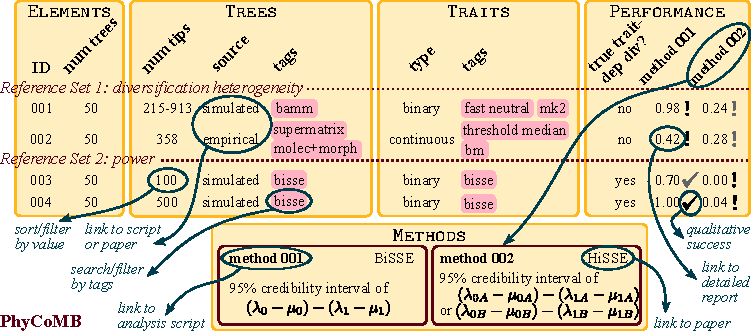
\includegraphics[width=\textwidth]{images/proposed}
\caption{
Vision for \phycomb.
The Phylogenetic Comparative Methods Benchmark database will provide test datasets and reports of method performance.
Example annotations are shown for four elements (comprising trees and traits), and interactive behavior of the web interface is noted.
Compared are two methods, which test for trait-dependent diversification by assessing the difference in estimated net diversification rates.
Performance is reported as the proportion of trees on which significant trait-dependent diversification is inferred.
Reference set 1 reveals the BiSSE-based method is prone to incorrectly associate two kinds of neutral traits with diversification rate, while the HiSSE-based method is less so.
Reference set 2 reveals that HiSSE has much lower power than BiSSE in this test.
(Note that HiSSE is much more effective under model averaging; \citealt{beaulieu2016}.)
}
\label{fig:proposal_phycomb}
\end{figure}

\bibliography{refs}
\bibliographystyle{nsf}

\subsection{Later thoughts}

This subsection wasn't part of the proposal.
But it explains some ways in which the current plan differs from what was proposed.

\bigskip

\textit{Task} needs to be defined a bit more carefully.
For example, even within the realm of state-dependent diversification, one approach/question is hypothesis testing and another approach/question is parameter estimation.
Results for those questions would be reported differently.
And even a given method on a given element could perform better on one question than the other.
Below, \textit{Task} is assumed to include this refinement.
But we could instead have a separate \textit{Question} component that intersects with \textit{Task} to specify the problem.

If we are going to include methods that co-infer the phylogeny along with answering the comparative methods question, we'd need to allow for input data to be a sequence alignment rather than a tree.
That is a potentially promising direction for methods development, but it's beyond the immediate scope of \phycomb.
